\section{Type classes}
\label{sec:typeclasses}

The first part of this section will give a short description of the concept of a type class. The second part will describe monoids in general and the type class \verb|Monoid|. The example in section \ref{sec:example} will prove a monoid type class law. 

The concept of a type class was introduced as a construct that supports overloaded functions and \emph{\gls{adhoc_polymorphism}} \cite{Wadler}. Overloaded functions can be used at a variety of types, but with diffenrent definitions at the different types. For example, the function calls \verb|show 1| and \verb|show "hello"| use different \glspl{function-definition} \verb|show 1| is of type \verb|Int -> String| and \verb|show "hello"| is of type \verb|String -> String|. The definition used depends on the type of the argument.  The next section will describe \gls{adhoc_polymorphism} and the relation to type classes in more detail.

\subsection{Polymorphism and type classes}
\label{sec:polymorphism}
%%In this section we will describe relation between type classes and polymorphism.
There are two types of polymorphism in Haskell \cite{Cardelli}: Parametric polymorphism and a \gls{adhoc_polymorphism}. Type classes are used for \gls{adhoc_polymorphism}.
\begin{description}
\item[Parametric polymorphism] Refers to a functions which work over more than one type. For example the library function \verb|length| returns the length of a list, that contains items of arbritrary type. It can be used to calculate the length of a list of integers, a list of strings, a list of booleans e.t.c. There are no constraints. The type of \verb|length| is
\begin{verbatim}
length :: [t] -> Int
\end{verbatim}
\verb|t| is a \emph{type variable}. That is, for any type \verb|t| the function \verb|length| has type \verb|[t] -> Int|. A type that contains a type variable is called \emph{polymorphic}. Hence, \verb|length| is a polymorphic type.
The \verb|length| function can be used with any type but it has a \emph{single} definition.  At compile time, the type variables are substituted with a concrete type. For example
\verb|[Int] -> Int|. 
\item[Ad hoc polymorphism] It's a synonym for function overloading or operator overloading. A overloaded function uses different function definitions depending on the types of the arguments. Suppose we want to define a function that converts a list containing items of arbitrary type (\verb|[t]|) to a string. We would write a function with the following type signature declartion.
\begin{verbatim}
showlist :: [t] -> String
\end{verbatim}
It takes a list of arbritrary type and returns a string. The defintion could look like this:
\begin{verbatim}
showlist [] = ""
showlist (x:xs) = show x ++ showlist xs
\end{verbatim}
We need a way to make sure that the function \verb|show| is defined for the type of the value \verb|x|. \verb|show| can't be a polymorphic type because the conversion depends on the type. There's no single definition that can convert an arbritrary type to a string. 

There's a set of types. \verb|show| is defined over all members of this set. This set is called a type class. The type class \verb|Show| for example contains all types that can be converted to a string with the function \verb|show|. In order to prevent the application of the function \verb|showlist| with a argument that isn't a member of the type class \verb|Show|, we must constraint the type variable in the type signature declaration \verb|t|:
\begin{verbatim}
showlist :: Show t => [t] -> String
\end{verbatim}
\end{description}

A type class is a collection of types. Certain functions declarated by the type class are defined over all members of the type class. And certain type classes exhibit properties that every definition of the corresponding functions must obey.

\subsection{Monoid}
\label{sec:monoid}

In mathematics, a \gls{monoid} is an algebraic structure with single associatve binary operation and an identity element. Monoids are semigroups with identity \cite{wiki:monoid}. Several elements of a monoid can always be reduces to a single element by applying the corresponding binary operator. It doesn't matter in which order we apply the operator, the result is always the same. This is called \emph{\gls{associativity}}. The set of elements has an identity element. For example, the set numbers form a monoid under multiplication. The number 1 is the identity element. Multiplication of the identity, the number 1, and any other number $x$ results always in $x$.

In Haskell there is a type class for monoids. Type that form a monoid can become part of the \verb|Monoid| typeclass. The example in section \ref{sec:example} shows a plugin system, that contains a monoid. Plugins can be composed with a binary operator. An arbritrary number of plugins can be composed to a single plugin. The order the plugins are added doesn't matter (\gls{associativity}). 

\subsubsection{Functions of the type class monoid}

Members of the type class \verb|Monoid| have to implement the functions \verb|mempty| and \verb|mappend| amongst others.

These functions have the following type signature declaration. The type variable \verb|m| is the type of the corresponding monoid.
\begin{verbatim}
    mempty :: m
    mappend :: m -> m -> m
\end{verbatim}

\verb|mempty| returns the identity value. The binary function is \verb|mappend|. It takes two values of the same type and returns another value of that type. 

The type class \verb|Monoid| exhibit serveral laws. We will only describe the one that we will prove in the example of section \ref{sec:example}. It called the \emph{left idendity law}.
When making monoid instances, we need to make sure that \verb|mempty| acts like the identity with respect to the \verb|mappend| function. This property can be expressed with the following equation:
\begin{equation}
  \label{eq:firstmonoidlaw}
  \text{mappend}(\text{mempty}, x) = x
\end{equation}

\subsubsection{Example monoid implementation}

There is a useful property of the \verb|Applicative| type class with respect to the \verb|Monoid| type class (the \verb|Applicative| type class is described in more detail in the appendix, section \ref{sec:applicatives}). The example in section \ref{sec:example} will use this property. If \verb|f| is an \verb|Applicative| and \verb|b| is a \verb|Monoid|, \verb|f b| is also a \verb|Monoid|. If a type is part of the \verb|Applicative| type class we can create a \verb|Monoid| instance with the implementation in listing \ref{lst:monoidinstance1}. Figure \ref{fig:applicative_monoid} illustrates the property.

\begin{figure}
  \centering
     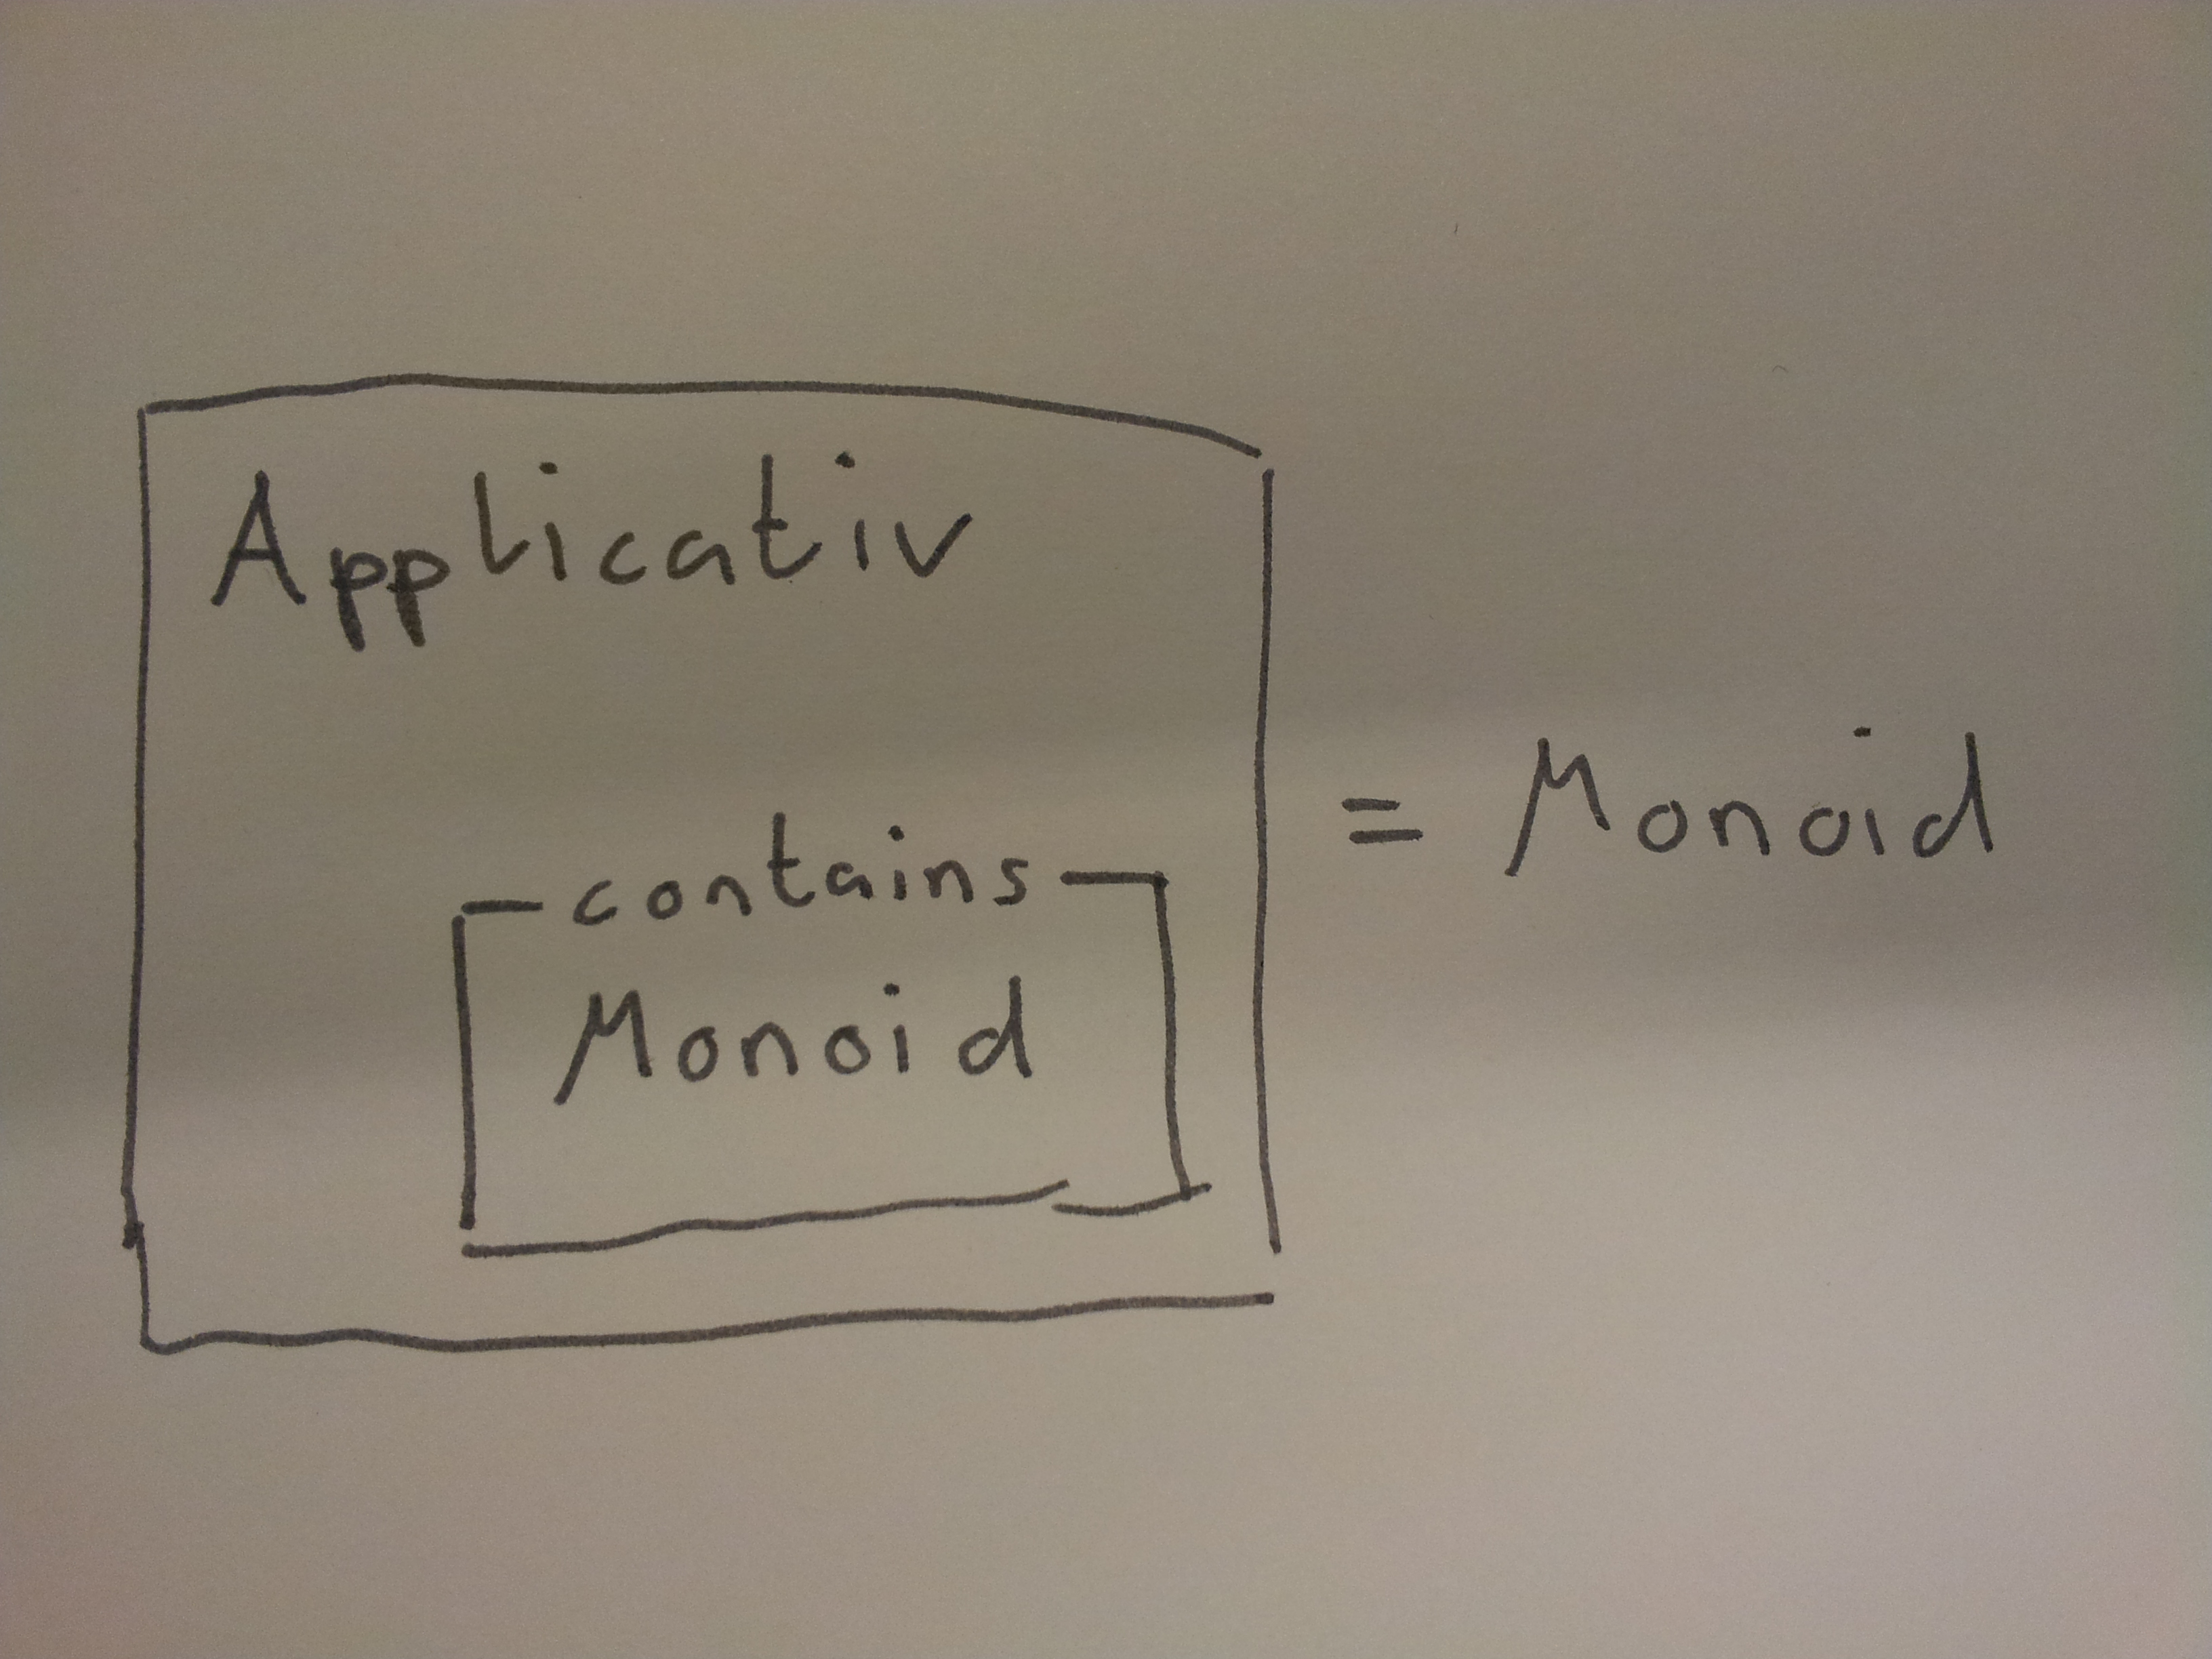
\includegraphics[width=0.9\textwidth]{applicative_monoid}
  \caption{An Applicative that encapsulates a monoid is a monoid}
  \label{fig:applicative_monoid}
\end{figure}

\lstset{
basicstyle=\ttfamily,
columns=fullflexible,
keepspaces=true,
}
\begin{lstlisting}[caption={Monoid instance implementation of applicatives},label={lst:monoidinstance1}]
instance (Applicative f, Monoid b) => Monoid (f b) where
    mempty = pure mempty
    mappend = liftA2 mappend
\end{lstlisting}

\verb|mempty| is of type \verb|f b| . Hence \verb|pure mempty| has to be of type \verb|f b|.
As \verb|f| is an applicative, it implements \verb|pure|. The type of \verb|pure| is \verb|a -> f a| (see \ref{sec:applicatives}). We call \verb|pure| with \verb|mempty|. When instantiated the type of \verb|pure| becomes \verb|b -> f b|.  We know that \verb|b| is part of \verb|Monoid| because of the type constraints. The compiler will use \verb|mempty| of \verb|b|.  \verb|liftA2| is an utility function of \verb|Applicative|. It encapsulates the \verb|mappend| function in an applicative functor. 

In section \ref{sec:example} we prove that the \gls{function-definition} of listing \ref{lst:monoidinstance1} obeys the first monoid law formed by equation \ref{eq:firstmonoidlaw} with  the verification technique equational reasoning.


